%
\documentclass[a4paper,12pt,twoside]{article}
\usepackage{iftex}

%% Разрешить компиляцию только с движком LuaTex
\ifLuaTeX
\else
    \newlinechar 64\relax
    \errorcontextlines -1\relax
    \immediate\write20{@
        ************************************************@
        * LuaLaTex is required to compile this document.@
        * Sorry!@
        ************************************************}%
    \batchmode\read -1 to \@tempa
\fi

%% Для русификации достаточно подключить пакет fontspec и
%% выбрать Unicode шрифт в котором есть кириллические глифы. Ниже
%% основным шрифтом выбирается Unicode версия шрифта Computer Modern с заcечками
\usepackage{fontspec}
\setmainfont{CMU Serif}
\setsansfont{CMU Sans Serif}
\setmonofont{CMU Typewriter Text}

%% В XeLaTex или LuaLaTeX альтернативой известного пакета babel является пакет polyglossia.
%% Теперь у нас будут переносы слов
\usepackage{polyglossia}
\setdefaultlanguage{russian}
\setotherlanguage{english}

\usepackage[autostyle]{csquotes} % Правильные кавычки в зависимости от языка
\usepackage{totcount}
\usepackage{setspace}

% ToDo:
% [] MathNote   : \sum[] syntax
% [] MathNote   : \tikzmatrix 
% [] Layout     : A4 geometry
% [] Layout     : Define colors
% [] References : Load knowledge
% [] References : Create simple clever refs
% [] Fix hidding enviroment

%Отключить предупреждения об кастномной использовании пакетов "You have requested package..."
\usepackage{silence}
\WarningFilter{latex}{You have requested package}

\usepackage{xparse}
\usepackage{configuration/floats}
\usepackage{configuration/layout}
\usepackage{configuration/references}
\usepackage{configuration/mathnote}

\sloppy
% Окружения для набора задач
\newcounter{boxlblcounter}  

\newcommand{\task}[1]{\fbox{\begin{minipage}{4em}\centering\it #1\end{minipage}}}
\newcommand{\makeboxlabel}[1]{\fbox{\begin{minipage}{2em}\centering\it #1\end{minipage}}\hfill}% \hfill fills the label box
\newenvironment{tasklist}
  {\begin{list}
    {\arabic{boxlblcounter}}
    {\usecounter{boxlblcounter}
     \setlength{\labelwidth}{3em}
     \setlength{\labelsep}{0em}
     \setlength{\itemsep}{2pt}
     \setlength{\leftmargin}{1.5cm}
     \setlength{\rightmargin}{2cm}
     \setlength{\itemindent}{0em} 
     \let\makelabel=\makeboxlabel
    }
  }{\end{list}}


\newboolean{ShowHint}
\newboolean{ShowSolution}

% Подсказка
\newcommand{\hint}[1]{\ifthenelse{\boolean{ShowHint}}{\noindent\rotatebox[origin=c]{180}{\noindent
\begin{minipage}[t]{\linewidth} \noindent \it Указание: #1 \end{minipage}}}{}}

% solution: окружение для набора решений
% solution*: форсировано показывает решение, независимо от флага
\makeatletter
\newenvironment{solution*}[1][\text{Решение}]{ 
  \par
  \pushQED{\qed}%
  \normalfont
  \topsep0pt \partopsep3pt
  \trivlist
  \item[\hskip\labelsep
    \itshape
    #1\@addpunct{.}]\ignorespaces
}{
  \ifthenelse{\boolean{ShowSolution}}{
    \popQED\endtrivlist\@endpefalse
    \addvspace{6pt plus 6pt} % some space after
  }{\end{hidden}}
}
\makeatother

%https://tex.stackexchange.com/questions/533218/hiding-an-environment-that-contains-minted-code
%https://tex.stackexchange.com/questions/38150/in-lualatex-how-do-i-pass-the-content-of-an-environment-to-lua-verbatim
\RequirePackage{luacode}
\begin{luacode*}
do 
    function eat_buffer(buf)
        i,j = string.find(buf,"\\end{solution}")
        if i==nil then return "" else return nil end
    end
    function start_proccesing_solution(eat)
        if eat then luatexbase.add_to_callback('process_input_buffer', eat_buffer, 'eat_buffer') end
    end
    function stop_proccesing_solution(eat)
        if eat then luatexbase.remove_from_callback('process_input_buffer', 'eat_buffer') end
    end
end
\end{luacode*}
%https://tex.stackexchange.com/questions/537219/conditionals-inside-newcommand-with-empty-argument
%https://tex.stackexchange.com/questions/63223/xparse-empty-arguments
\ExplSyntaxOn
\DeclareExpandableDocumentCommand{\IfNoValueOrEmptyTF}{mmm}{\IfNoValueTF{#1}{#2}{\tl_if_empty:nTF {#1} {#2} {#3}}}
\NewDocumentCommand{\DefaultName}{mm}{\IfNoValueOrEmptyTF{#1}{#2}{#1}}
\ExplSyntaxOff

% WARNING!
% Buggy: one have always have
% \begin{solution}{NAME}
%   ....
% \end{solution}
% EVEN if NAME is empty
% if one starts some text on the same line as \begin{solution} or \end{solution} it could'not be hidden
\newenvironment{solution}[1]%
{
  \ifthenelse{\boolean{ShowSolution}}
    {\begin{solution*}[\DefaultName{#1}{\textit{Решение}}]\directlua{flag_eat=false}}
    {\directlua{flag_eat=true}}
  \directlua{start_proccesing_solution(flag_eat)}
}
{
  \ifthenelse{\boolean{ShowSolution}}{\end{solution*}}{}
  \directlua{stop_proccesing_solution(flag_eat)}
}


\newcommand{\PracticeSubject}{}
\newcommand{\PracticeGroup}{}
\newcommand{\PracticeCourse}{}
\newcommand{\HWname}{}
\newcommand{\HWnumber}{}
\newcommand{\Deadline}{}

\AtBeginDocument{%
    % Метаданные:
    \title{\HWname}%
    \date{\today}%
    % Настраиваем колонтитулы
    \pagestyle{fancy}%
    \lhead{\PracticeGroup, курс \PracticeCourse}%
    \chead{\PracticeSubject. ДЗ №\HWnumber}%
    \rhead{Дедлайн: \Deadline}%
    % Название практики
    \section*{\strtitle}
}
\mmzset{memo dir = images/cache/\jobname}


\setboolean{ShowHint}{false}
\setboolean{ShowSolution}{false}

\renewcommand{\PracticeSubject}{Дискретная математика}
\renewcommand{\PracticeGroup}{ПМИ}
\renewcommand{\PracticeCourse}{2}
\renewcommand{\HWname}{ДЗ №1, разминочное}
\renewcommand{\HWnumber}{1}
\renewcommand{\Deadline}{29 янвая в 23:59}

\begin{document}
\begin{?}[Разминочная]\ \\
    \task{1 балл} 
    В связном графе степени четырех вершин равны 3, а степени остальных вершин равны~4. Докажите, что нельзя удалить ребро так, чтобы граф распался на две изоморфные компоненты связности.
\end{?}
\begin{?}[Про деревья -- 1]\ \\
    \task{1.5 балла}
    Пусть $G$ --- простой граф с $\delta(G)\geq k$, а $T$ --- произвольное дерево с $k$ ребрами. Докажите, что в $G$ имеется подграф, изоморфный $T$.
\end{?}
\begin{?}[Про деревья -- 2]\ \\
    \task{1.5 балла}
    Пусть $G$ --- простой граф, построенный на $n$ вершинах и имеющий более $n(k -1) - \binom{k}{2}$ ребер, а $T$ --- произвольное дерево с $k$ ребрами. Докажите, что в случае $n > k$ в графе $G$ имеется подграф, изоморфный $T$
\end{?}
\begin{?}[Лемма Шпернера]\ \\ 
    \task{2 балла}
    Дан треугольник, вершины которого помечены цифрами 0, 1 и 2, и его триангуляция. Вершины триангуляции пометили теми же значениями таким образом, чтобы любая вершина на стороне исходного треугольника была бы помечена одной из пометок вершин этой стороны. Докажите что обязательно существует треугольник разбиения, помеченный цифрами 0, 1, 2. 
    
    \begin{figure}[h!]
        \begin{center}
            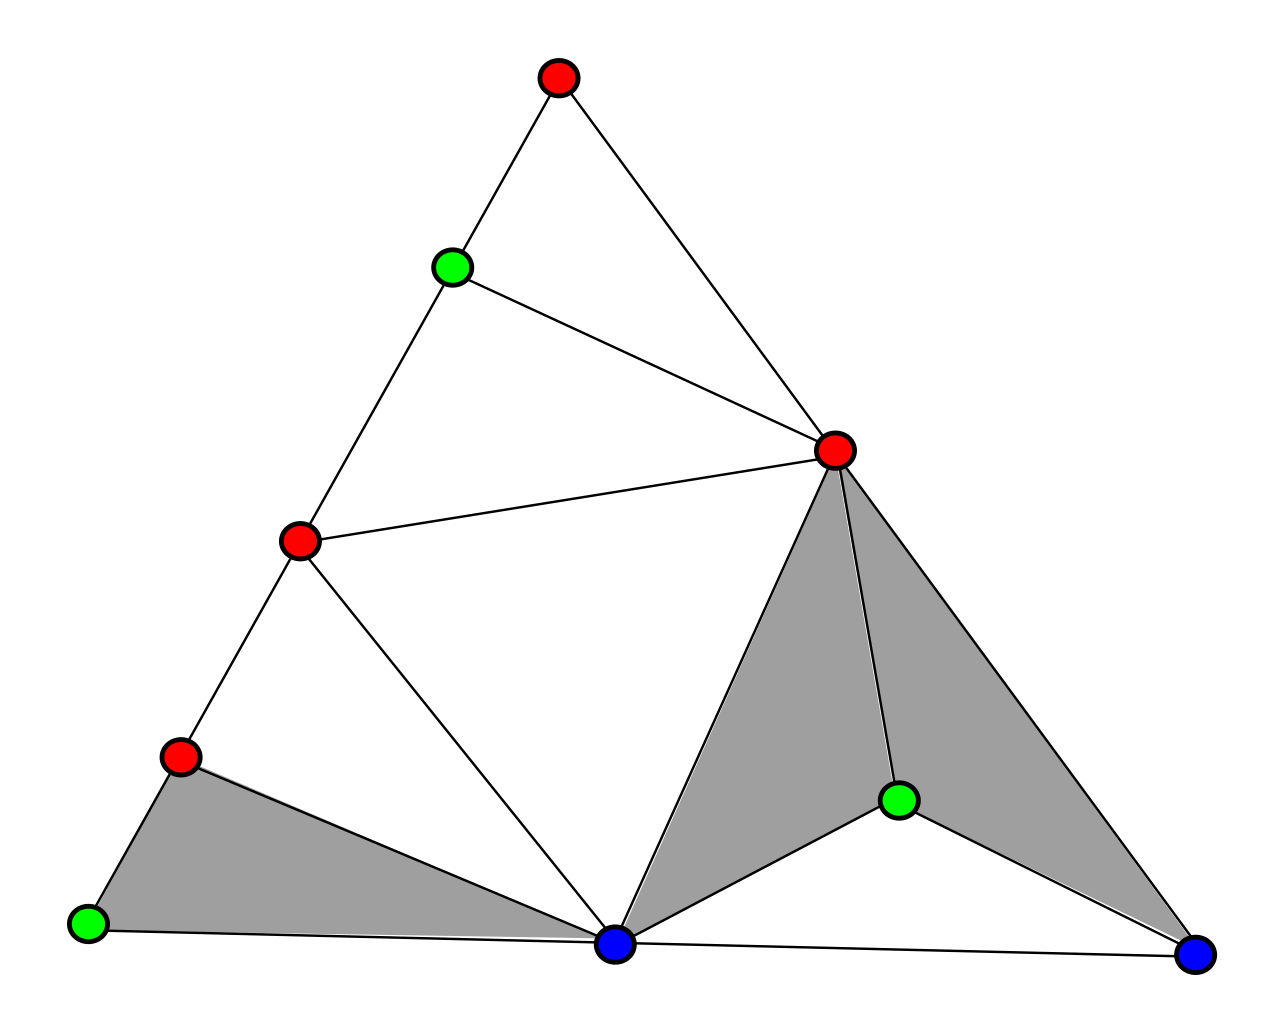
\includegraphics[scale=0.1]{images/homeworks-01-sperner}
        \end{center}
    \end{figure}
\end{?}
\begin{?}[Нетривиальная задача]\ \\
    Обхватом графа $G$ называется длина наименьшего цикла, содержащегося в $G$.
    \begin{tasklist}
        \item[0.5] Докажите что величина
        \[
            D(G) \coloneqq \sum_{v \in V(G)} \binom{\deg v}{2}
        \]
        есть число троек вершин \((u, v_1, v_2)\) таких что \(u \in N(v_1) \cap N(v_2)\) (тройки \((u, v_1, v_2)\) и \((u, v_2, v_1)\) считаются одинаковыми)
        \item[1] Докажите, что если \(V(G) = n\) и
        \(
            D(G) > (l - 1) \binom{n}{2}
        \),
        то граф \(G\) содержит \(K_{2, l}\) в качестве своего подграфа.
        \item[1.5] Докажите что в графе с \(|V(G)| = n\) и \(|E(G)| = m\) имеет место следующее неравенство:
        \[
            D(G) \geq \frac{m \cdot (2m - n)}{n}
        \]
        \item[1] Докажите, что обхват графа \(G\), построенного на \(n\) вершинах и имеющего более чем \(\tfrac{1}{2}n \sqrt{n - 1}\) ребро не превосходит 4.
    \end{tasklist}
\end{?}
\end{document}

